% Documento creado por �scar Varela Su�rez y Jos� Antonio Almena Mu�oz
% Haz con �l lo que quieras...

% si queremos que un cap�tulo nuevo empiece en cualquier p�gina (dcha. o izda.) ponemos dentro de las
% opciones de documentclass --> openany
\documentclass[twoside,a4paper,12pt]{book}

\usepackage[dvips]{graphicx}
\usepackage[spanish]{babel}
%\selectlanguage{spanish}
%\usepackage[T1]{fontenc}
\usepackage[latin1]{inputenc}
\usepackage{babel}
\usepackage{fancyhdr}
\usepackage{caption2}
\usepackage{geometry}
\usepackage{makeidx}
\usepackage{graphicx}
\usepackage{hthtml}
\usepackage{latexsym}
\usepackage{amssymb}
\usepackage{eucal}
\usepackage{setspace}\singlespacing
% Para otros interlineados: \renewcommand{\baselinestretch}{1.05}
\usepackage{dsfont} %Para las formulitas

%\pagestyle{headings}

\geometry{left=2.5cm, right=2.5cm, top=2.5cm, bottom=2.5cm}

%para crear un �ndice alfab�tico (de usarlo lo hacemos al final del documento)
\makeindex

\begin{document}

\renewcommand{\captionlabelfont}{\textbf}

\pagestyle{fancy}

\fancyhf{}
%
\renewcommand{\headrulewidth}{0.5pt}

\fancyhead[LO]{\rightmark} % En las p�ginas impares, parte izquierda del encabezado, aparecer� el nombre de cap�tulo

\fancyhead[RE]{\leftmark} % En las p�ginas pares, parte derecha del encabezado, aparecer� el nombre de secci�n

\fancyhead[RO,LE]{\thepage} % N�meros de p�gina en las esquinas de los encabezados
%

% para no numerar la p�gina
\thispagestyle{empty}

% si se comenta la siguiente l�nea en el encabezado de una pagina aparece el cap�tulo al que pertenece en lugar
% de la secci�n a la que pertenece
\baselineskip 1.35\baselineskip

\vspace{2cm}
%
\begin{figure}[htb]
%%Escudo de la reyjuan
%Para que inserte la imagen en el pdf ejecutar DVI2DPF
\centerline{\resizebox{.05\textwidth}{!}{\includegraphics{logo_urjc.eps}}}
\end{figure}
%
\begin{center}
{\Large {\bf Universidad Rey Juan Carlos}} \vspace{5mm}

%
{\large Escuela Superior de Ciencias Experimentales y Tecnolog�a}
\vspace{5mm}

%
{\large Departamento de Inform�tica, Estad�stica y Telem�tica}

%
\vspace{4.5cm}
%
%
%

{\Large {\bf ------ t�tulo ------}}

\vspace{3cm}

%
{\large {\bf Trabajo Fin de Carrera}}
%
%
\vspace{4cm}


--- Autor ---\\
\vspace{1cm}
---Tutor---\\
\vspace{1cm} \today

%
\end{center}
%Para que nos deje una p�gina en blanco despu�s de la portada
\newpage{\pagestyle{empty}\cleardoublepage}


\setcounter{page}{1} %para que no cuente la primera p�gina (la portada)
%\setcounter{secnumdepth}{2} \setcounter{tocdepth}{2}


% el documento est� desglosado en diferentes ficheros
% para incluir cada uno de ellos en el total se utiliza la sentencia: \include{nombre_fichero}

% para que no ponga "Cap�tulo 0" en las secciones agradecimientos y resumen
\renewcommand{\chaptermark}[1]{\markboth{\small{\  #1}}{}}

\frontmatter

% ----------------- AGRADECIMIENTOS --------------------
\chapter{Acknowledgments}
%\thispagestyle {empty}

Acknowledgments to my mentor, Manuel Rego. 
To Ram\'on Castro P\'erez who helped me to run Siestta work. 
To Jos\'e Manuel Ciges Regueiro, which memory I used as a template for my own work, and every 5th Master Software Libre classmate.          

% ----------------- RESUMEN ----------------------------
\chapter{Description of the practicum}
%\thispagestyle {empty}
The main objective of this Master Thesis consist in the development of an mobile application to be used int highschools by teachers.
It could allows teachers to carry on control students attendance, their behavior. Also it permits quick assessment by activity.
Teachers would read students reports: weekly and daily assessment, by activity assessments and total marks.
\begin{itemize}
  \item {Name :} Jos\'e Antonio Salgueiro Aquino.
  \item {Birth date: } august 5th 1970
\item {Education:} B.Sc. in Fundamental Physics, University of Santiago de Compostela University 1988-1993.
\item {Address:} Marin (Pontevedra). Spain.
\item {Current position: } Secondary School teacher in Technology.
\end{itemize}

\begin{itemize}
  \item {Working times :} (planned) 300 hours. 	From 6th August, to 30 September, on an eight hours day basis.
\end{itemize}
Working times (planned): 300 hours.

This application involves several technologies:
Java language.
Android skeleton application.
PhoneGap framework to develop multi-platform applications.
JQuery and JqueryMobile  to develop mobile oriented applications.
JavaScript with Web Databases.
Git for version control system.
Meetings:
	One meeting on August: Technologies to be used were stated, work methodologies, first application windows (pages), Android version to be used (2.3.3) because is the most popular. 
	Several emails and gtalk conversations about organization, general problems were written.
Teleworking is done. 
Materials and special equipment used:
	For main development: 
Hardware: Intel Quad, 6GiB RAM, 500GiB HD. 

Software: Debian Linux Wheezy (testing), Eclipse Juno, JQuery 1.8.1, jQueryMobile 1.1.1, and PhoneGap-Cordova 1.8.1, Android Virtual Manager 2.3.3, Git 1.7.10.4-1.
For testing Sony-Ericsson Xperia V mobile phone, with USB cable.
    
    


% para que vuelva a poner "Cap�tulo n" donde corresponda a partir de esta l�nea
\renewcommand{\chaptermark}[1]{\markboth{\small{\chaptername \ \thechapter. #1}}{}}
% ----------------- �NDICE GENERAL ---------------------
\tableofcontents
% ----------------- �NDICE DE FIGURAS ------------------
\listoffigures

\mainmatter

% ----------------- INTRODUCCI�N -----------------------
\chapter{Introduction}
In a high school, there are classes which attendance, assessment and group dynamics is difficult to control.
This is especially relevant for the technology workshop, this could be a noisy, annoying, even dangerous place, which requires teacher's standing monmitoring.
 This workshop needs a lightweight,
reliable and also complete  software tool. A simple web solution is not enough, because it could be too complicated and not fast enough; even use a tablet can be heavy. Therefore, this problem requires a new approach.
  
The development of a multiplatform tool, open source, for smartphones, including tablets, for attendance monitoring and evaluation of students is suggested.
 To achieve this goal a client-side application will be developed using a multiplataform framework: Phonegap (Cordova) \cite{PhoneGap}.
Phonegap allows you to develop quickly, utilizing well-known languages as Javascript and HTML. It permit us to deploy an application for both
 Android, WebOS, iOS and others.    

For data management, a built-in database, SQLite, will be employed which has all capabilities needed (autoincremental indexes, relation among tables and several built-in functions ).
  
The tool that enables rapid development of the application and integration of performance tests is Eclipse. Also Eclipse is well integrated with Android SDK, and its Android virtual machine (AVM).

% ----------------- ESTADO DEL ARTE --------------------
\chapter{State-of-art solutions}


	Only an open source application was found for study, Siestta  ,  nevertheless there are a lot of educational software (Sixa2, Unisoft3) but they are privative, Microsoft Windows freeware or both (SAS acad�mico4). 
	Siestta was evaluated. 
Technically it is an GPL'ed old style PHP-based web application with Ajax, an interactive editor, fckeditor and fpdf to generate reports.
From user point-of-view there are online documentation5. This application includes management of students, attendance, marks, tasks, incidents, general queries, letters to parents, interviews with parents, messages, appointments, exams and more.
	Several screen-shots were taken and will be reused in current application:


\section{Siestta}

This application (Siestta) are also available for PDAs, it could be a valid solution but it is server-side with outdated technologies. Data structure from Siestta is standard and fully functional, and it could be partially reused by EduXes.
Source code are also shown: calendario.php. It shows us a PHP application which uses sessions variables and is not Model-View-Controller oriented.

\fcolorbox{black}{gray!20}{
\parbox{\tw}{All parts of this prealgebra textbook are copyrighted � 2009 in the name Department of Mathematics, College of the Redwoods. They are not in the public domain. However, they are being made available free for use in educational institutions. This offer does not extend to any application that is made for profit. Users who have such applications in mind should contact David Arnold or Bruce Wagner at [hidden email] or [hidden email].
}} 


\begin{minipage}[c]{200pt}
 text text
 \end{minipage}




\begin {shaded}
\begin{verbatim}
<?php 
session_start(); 
require('config.php'); 
require('idioma/'.$idioma.''); 
include('funciones_calendario.php'); 
$docente = $_SESSION['usuario_sesion']; 
//recogemos variables 
$mes_actual = $_POST['mes']; 
$anyo_actual = $_POST['anyo']; 
if($mes_actual || $anyo_actual) { 
	include('funciones.php'); 
	conecta(); 
	} 
//si es la primera vez que entramos, cargamos la fecha actual 
if(!isset($mes_actual)) $mes_actual = date('m'); 
if(!isset($anyo_actual)) $anyo_actual = date('Y'); 
//presentamos ahora el calendario del mes actual o cargado 
//tabla con nombre mes y a�o y las flechas para navegar 
echo ' 
<br /> 
<table class="tablacentrada_i"> 
<tr> 
<td> 
<a href="#" onclick="navegaMes(\''.$mes_actual.'\',\''.$anyo_actual.
'\',\'menos\')" title="'.$id_anterior.'"><img src="imgs/anterior_peq.png" 
class="alin_bajo" alt="'.$id_anterior.'" /></a> 
'; 
$nombre_mes = numero_mes_a_nombre($mes_actual);
\end{verbatim}

\end{shaded}

Develop database structure: tables and relationships. 
Data base structure looks like Illustration 5: EduXes Database structure 


\section{Sixa}

\section{Other Android applications}
\subsection{Grade Book}
https://play.google.com/store/apps/details?id=com.gradebook.academics
Description
Now teachers can manage their students grades directly on their Android device!
Key Features:
-No need to sync two separate grade books! Use one primary grade book on Google Spreadsheets
-Email student grades with the click of a button
-Pin-number to protect your grade books if your phone is lost
Instructions at website
keywords: gradebook, grading, grades, grading tools, grade, grade tools
Updated:
    July 7, 2011
Current Version:
    1.07
    Price  4  \geneuro 
 
\begin{figure}
    \begin{center}
        \includegraphics[scale=0.5]{grade_book01.jpg}
        \caption{Grade Book}
        \label{fig:Grade Book}
    \end{center}
\end{figure}

\subsection{Attendance}
https://play.google.com/store/apps/details?id=com.academics.attendance
Attendance

A great way to take attendance. Put your student list in a Google Spreadsheet, and this app takes care of the rest. There is no need to enter total absences into a spreadsheet at the end of the semester because all absences/tardies are calculated in your google spreadsheet each day you take attendance.

HOW-TO on website: http://androidforacademics.com/2010/09/attendance-instruction-manual/

Keywords: attendance
Price: Free
\begin{figure}
    \begin{center}
        \includegraphics[scale=0.5]{attendance01.png}
        \caption{Attendance}
        \label{fig:Attendance}
    \end{center}
\end{figure}




\subsection{ Teacher Organizer }

https://play.google.com/store/apps/details?id=com.sorokinkirill.teacherorganizer
Gradebook and attendance, notes, schedule a teacher (high school teacher)

Unified information resource teacher developed within diploma projects.

Implemented the following functionality:
1. functional log attendance and log evaluations point system of evaluation, while allowing classes to celebrate and stand missing the mark;
1.1. compilation of the magazine is "on the fly", depending on the selected students;
1.2. selection of students by selecting a training group, not the individual student;
1.3. Log open it is possible to select more than one group of students;

2. entering information about your child and watching it like when viewing the log evaluations or visits, and without the need to open the log;

3. notebook;
3.1. notebook allows you to store notes, view, and edit;
3.2. a system for cataloging notes for quick search;
3.3. The possibility of entering one note in more than one subject group;

4. schedule a private teacher;
4.1. it is possible to view the schedule for the next semester as up to now, and after;
4.2. the system can generate the schedule for a few weeks in advance, if it is repeated;
4.3. supports two-week schedule (odd and even weeks).

Home Page: http://4pda.ru/forum/index.php?showtopic=345457\&st=80
Program in Russian

Price : Free
This seems to be very professional.

\begin{figure}
    \begin{center}
        \includegraphics[scale=0.5]{teacher_organizer01.jpg}
        \caption{Teacher Organizer}
        \label{fig:TeacherOrganizer}
    \end{center}
\end{figure}





\subsection{Teacher Aide  }

https://play.google.com/store/apps/details?id=com.glen.apps.TeacherAideProLite

This is a free DEMO version of the Teacher Aide Pro app. The app allows teachers to take attendance and record grades on their phone or tablet. The main features are listed below.

The Lite version only allows the user to keep data for 5 students per class - otherwise all functionality is present so the user can truly test out the app before purchasing the PRO version

Features
- default values set to Present for fast attendance
- import student names via CSV file
- export data via CSV generated file send via email or to Dropbox (THE CLOUD)
- 1-click text to students/parents for tardy/absent students and missing assignments.
- 1-click Random student generator (no more popsicle sticks)
- Grading interface to allow recording of assignments using Yes/No/Missing, Points, Letter Grades, Percent.
- Generate PDF file for attendance and grade reports.
- Print reports directly to Google Cloud Printer from app.

New Features added all the time.

Explanation for some Permissions
SMS-Allows user to send bulk text message to parents and students
CALL Phone - Call parents/student right from the App
INTERNET - Send bulk email to parents/students from app without having to confirm 1 at a time
READ CONTACTS - Allows the user to save or load student/parent contacts from the device contact list. Your contact data is not read FOR ANY OTHER REASON, NOR TRANSMITTED OVER THE INTERNET.

I am a high school science teacher in the San Francisco Bay area.
Feedback or to inpocketsolution@gmail.com

Keywords: Attendance, Teacher, School, Roster, SIS, Gradebook, grades, TA, Teacher assistant, professor, coaches, team, sport, grading, gradebook, gradebook, schoolloop



Excellent but not free.

\begin{figure}
    \begin{center}
        \includegraphics[scale=0.5]{TeacherAideProLite01.jpg}
        \caption{Teacher Aide}
        \label{fig:TeacherAide}
    \end{center}
\end{figure}




Bas�ndose en art�culos, libros, etc. que se os haya facilitado y
de otros que estim�is oportuno, se hablar� de:
\section{Descripci�n del problema}
\dots
\section{Descripci�n de los trabajos anteriores que se han dedicado a resolverlo}
\dots

% ----------------- OBJETIVO ---------------------------
\chapter {Objetivo (5\%)}

\section {Descripci�n, en un objetivo general, de la finalidad del proyecto.}
\dots
\section {Descripci�n de objetivos parciales que se necesitan cubrir para llegar al objetivo final}
\dots
\section {Descripci�n de alto nivel de las etapas que sigues en el desarrollo}
\dots

% ----------------- DESCRIPCI�N INFORM�TICA ------------
\chapter{Descripci�n Inform�tica (20-35\%)}


Preparation of development:
 a) Build development environment: 
Java Development Kit (JDK) version 1.6 is downloaded from: 
http://www.oracle.com/technetwork/java/javase/downloads/index.html
As root user that file is unpacked into /usr/lib/jvm and configured to be the Java default:
\begin{verbatim}
 # update-java-alternatives -s JDK_1.6_NAME
\end{verbatim}  
	Eclipse Juno (4.6) is downloaded from its web-page:
http://www.eclipse.org Download->Linux 64 bits
Android Development Toolkit (ADT) is downloaded following instructions on this page:
http://developer.android.com/sdk/installing/installing-adt.html 
	A new line is included into repository software (Help ->  Install New Software -> Add):
http://dl-ssl.google.com/android/eclipse/
	Next step is to select all the related software listed.
	For Aptana Plugin line to add into Eclipse is: 
http://download.aptana.com/studio3/plugin/install
	Furthermore JQuery, JQueryMobile and Phonegap are needed, and were downloaded from their web sites:
JQuery 1.8.1 (no newer versions):
http://jquery.com/ 
JQuery will be  copied into assets/www/js folder.
JQueryMobile version 1.1.1 from
http://jquerymobile.com/ 
JQueryMobile is a zip file which will be uncompressed and copied into 
assets/www/js folder.
	PhoneGap - Cordova 1.8.1 is downloaded from this URL:
https://github.com/phonegap/phonegap/zipball/1.8.1 
	To create a PhoneGap application this very important instructions (Getting Started with Android)  should be followed step by step:
\cite{AndroidGettingStarted}

 b) Choose application name and folder's policy:
EduXes stands for "Educaci�n" and "Xesti�n", is a educational management software.
A folder is created (assets/www/js) which contains javascript (*.js) files except JQuery and JqueryMobile which is included into another folder (assets/www/js/jquery), do not forget style sheet files (*.css)
 c) Make a simple application: only a blank page.
Getting started with Android is followed step by step.
 d) Upload simple application into a git repository. 
A Github account is created and a new application is initialized.  This are the source code project page:\cite{EduXes}
Source code are upload to GitHub: 
  \begin{bclogo}[couleur=green!30,arrondi=0.1, logo=\bcpanchant,  ombre=true ] 
{Git init shell}   
\begin{verbatim}
$ git init
$ git add -A *
$ git remote add  EduXes git@github.com:joseantoniosa/EduXes.git 
$ git push origin master
\end{verbatim}
\end{bclogo}





\section{La base de datos coleccionada (si tiene sentido).}
\dots
\section{Los algoritmos para el desarrollo de la soluci�n}
\dots

\section {qu� quieres resolver}
\dots
\section {c�mo lo vas a hacer}
\dots
\section {herramientas conceptuales necesarias}
 \dots
\section {Tools}
%\chapter{Anexo 2}
These are several tools used to build these documentation:
\begin {itemize}
\item Sqlfairy. Tranforms SQL language into a  image in \emph{png} format.
\item LaTeXila 2.7.0 to write this document. 1 
\item Gimp 2.8.2 to get screen-shots.
\item GNU/Debian Wheezy tools  October 2012 .
\end{itemize}



\begin{framed}
  ASD
\end{framed}

\begin{shaded}
  FFG
\end{shaded}

\begin{ovalbox} 
{
OVAL BOX
}
\end{ovalbox}

%%     la fleur : commande \bcfleur
%%     en chantier  : commande \bcpanchant (Jean-Michel SARLAT)
%%     la note : commande \bcnote (Thomas LABARRUSIAS)
%%     l etoile : commande \bcetoile
%%     l ourson : commande \bcours
%%     attention  : commande \bcattention
%%     le cour : commande \bccoeur
%%     ornement : commande \bcorne
%%     danger : commande \bcdanger (Fran�ois BOERKMANN)
%%     smiley heureux : commande \bcsmbh (Fran�ois BOERKMANN)
%%     smiley malheureux : commande \bcsmmh (Fran�ois BOERKMANN)
%%     Take care : commande \bctakecare (Patrick FRADIN)
%%     Lampe : commande \bclampe (Patrick FRADIN)
%%     Le livre : commande \bcbook (Patrick FRADIN)
%%     Le trefle : commande \bctrefle


\begin{shadowblock}{16cm}
OVAL BOX shadowblock
\end{shadowblock}

%% logo=\bcrayon,
\begin{bclogo} [couleur=blue!30,arrondi=0.1,  ombre=true ] 
{Contenido}
, contenido ...
\end{bclogo}

% ----------------- RESULTADOS EXPERIMENTALES ----------
\chapter{Results}

Application is evolving from list, edit students and groups, to its final goals. These objectives were fulfilled:
\section{Objectives completed}
\begin{itemize}
  \item Access to any workday, any group and student.
  \item Management of attendance and misbehaviour of each student. The students information is still hard-coded into source files.
  \item 
\end{itemize}


\section{Technical details}
Javascript-SQL conexion
Asynchronous methods


\section{Further objectives}

\begin{itemize}
\item Links to student and group management. These pages were done but links are not missing into main application window.
\item There are several objectives not fulfilled yet, but I am on the way to get those done, those are, in priority order:
\item Data visualization. Student attendance and misbehaviour have to be shown in table-like window.
\item Test into real hardware. EduXes.apk has to be copied into mobile phone.
\item Activities evaluation per student. A window to display activities marks and final mark.
\item Timetable management. A window to manage groups timetable. When a group has class with this teacher.
\item Server synchronization with a custom application or

\end{itemize}

%%Como se desenvolveu o teu traballo, que obxectivos
%%> puideches acadar e cales non e porqu�. Inclu�r neste apartado a
%%> descrici�n da aplicaci�n desenvolvida, que � o que agora mesmo t�s no
%%> cap�tulo 4.Description.

These objectives were not fulfilled because time and skills lack.



En este apartado deber�n quedar reflejados los experimentos
realizados. Para ello se mostrar�n:
%% \cite{Cita}
\ref{fig:siestta30}
%% TODO: Screenshots:
\begin{figure}
    \begin{center}
        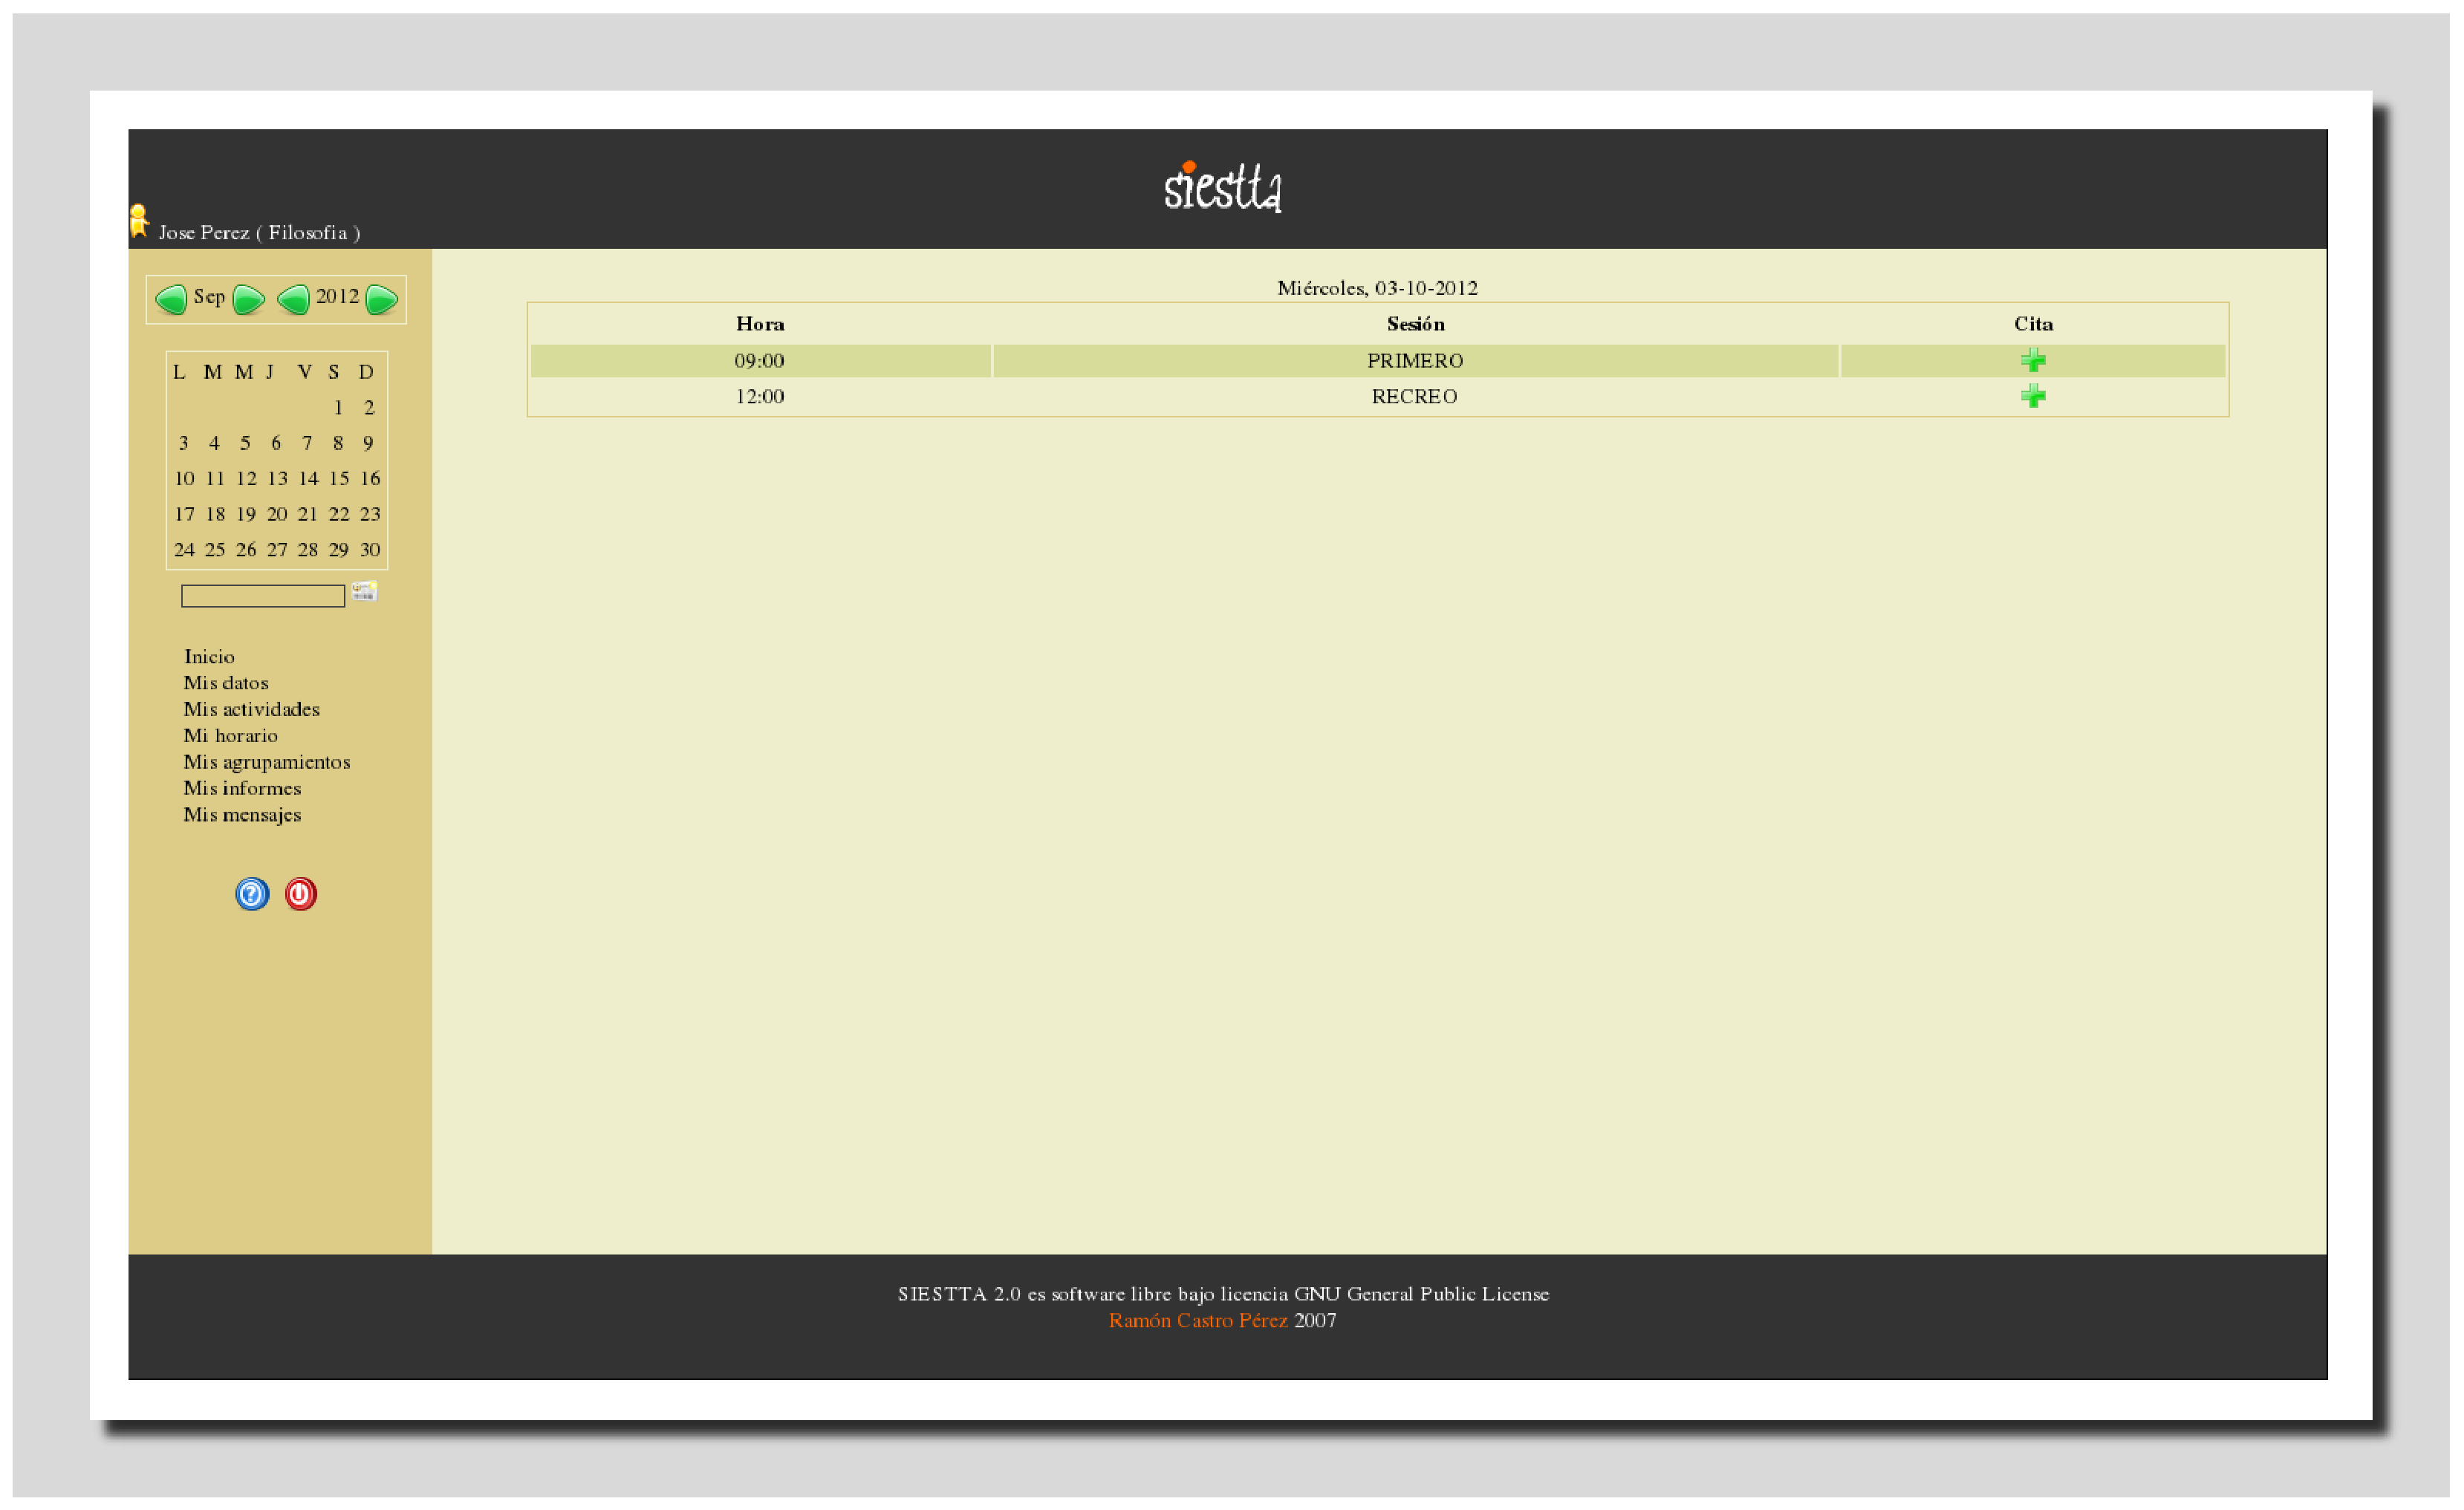
\includegraphics[width=\textwidth]{siestta2.eps}
        \caption{Siestta Main Page}
        \label{fig:siestta30}
    \end{center}
\end{figure}





\section {Resultados en forma de tablas, gr�ficas e im�genes donde se describa cuantitativa
            y cualitativamente el funcionamiento de la aplicaci�n} \dots

\section {An�lisis cr�tico de los resultados con el objetivo de decidir si el sistema implementado es v�lido}
\dots

Several problems were faced:
Eclipse environment: A stable, reliable and up-to-date IDE, with several plug-ins is needed. Download vanilla Eclipse Juno from its web-site is chosen because it is more stable, reliable, compatible with newer versions.  Aptana Javascript plugin was chosen because Aptana allows source code auto-completion in JQuery.
PhoneGap and Android incompatibilities. Android 2.3.3 requires JQuery-1.8.1 and does not work on higher versions. 
Error handlers. I have had several problems with tx.executeSql(...) function, it confused me with db.transaction(...): 
tx.executeSql(sql, [parameters],  successHandler, errorHandler)
and
db.transaction(queryFunction, errorHandler, successHandler)  
have up to four and three parameters respectively, only first one is mandatory. I rather use success and error handlers for tx.executeSql function, atomic error control could be better choice.
Passing variables to functions: Only if another solution is not known or feasible, global variables are used: named after global\_\*, and in block capitals.
Deadline. Development was delayed because I have no enough spare time and above problems were time costly.

\begin{verbatim}
 ohcount -i  assets/www/js/database.js assets/www/js/interface.js \
 assets/www/js/create_populate_db.js  assets/www/index.html \
 assets/www/remove.html 
Examining 5 file(s)
                              Ohloh Line Count                              
Language               Code    Comment  Comment %      Blank      Total  File
----------------  ---------  ---------  ---------  ---------  ---------  -----------------------------------------------
javascript             1374        155      10.1%        210       1739  database.js
javascript              393         91      18.8%         56        540  interface.js
javascript              402         57      12.4%         46        505  create_populate_db.js
html                    546         99      15.3%        117        762  index.html
javascript                1          0       0.0%          0          1  index.html
html                     28          1       3.4%          8         37  remove.html

\end{verbatim}

% ----------------- CONCLUSIONES Y TRABAJOS FUTUROS ----
\chapter{Conclusiones y trabajos futuros (5\%)}

Resumen de los logros principales conseguidos, destacando:

\section {Implementaci�n}
\dots

\section {Resultados}
\dots

En futuros trabajos, a partir de una cr�tica constructiva del
trabajo realizado, plantear mejoras y extensiones del mismo.


\backmatter

% para que no ponga "Cap�tulo n" en las secciones anexo y bibliograf�a
\renewcommand{\chaptermark}[1]{\markboth{\small{\  #1}}{}}
% ----------------- ANEXOS -----------------------------
\chapter{Anexo 1}
Lo relativo al anexo 1 \dots

Ejemplos de tratamiento de texto:

Probamos una cita \cite{NewCam97}\\
Citamos un libro\cite{Pesce}\\
Probamos a poner una nota al pi�\footnote{Mi primera nota al pi�}\\
Probando: \it{cursiva} \textbf{negrita} \underline{subrayada} \emph{enfatizar}\\


% pueden hacer falta varios anexos
%\chapter{Anexo 2}

% ----------------- BIBLIOGRAF�A -----------------------
    % para que funcione bien esto se debe compilar all� donde halla una cita usando "bibtext"
    % el "alpha" es para que ordene la bibliograf�a por orden alfab�tico
\bibliographystyle{alpha} \bibliography{librero}
% incluye la bibliograf�a en el �ndice
\addcontentsline{toc}{chapter}{Bibliograf�a}

%\printindex  %%%% crea un �ndice alfab�tico con las palabras indexadas en el documento: \index{palabra}

\end{document}
